% This is "TrustfullActionSuggestion-Paper" 
% Adapted from "sig-alternate.tex" V2.1 April 2013
% This file should be compiled with V2.5 of "sig-alternate.cls" May 2012
%
% This example file demonstrates the use of the 'sig-alternate.cls'
% V2.5 LaTeX2e document class file. It is for those submitting
% articles to ACM Conference Proceedings WHO DO NOT WISH TO
% STRICTLY ADHERE TO THE SIGS (PUBS-BOARD-ENDORSED) STYLE.
% The 'sig-alternate.cls' file will produce a similar-looking,
% albeit, 'tighter' paper resulting in, invariably, fewer pages.
%
% ----------------------------------------------------------------------------------------------------------------
% This .tex file (and associated .cls V2.5) produces:
%       1) The Permission Statement
%       2) The Conference (location) Info information
%       3) The Copyright Line with ACM data
%       4) NO page numbers
%
% as against the acm_proc_article-sp.cls file which
% DOES NOT produce 1) thru' 3) above.
%
% Using 'sig-alternate.cls' you have control, however, from within
% the source .tex file, over both the CopyrightYear
% (defaulted to 200X) and the ACM Copyright Data
% (defaulted to X-XXXXX-XX-X/XX/XX).
% e.g.
% \CopyrightYear{2007} will cause 2007 to appear in the copyright line.
% \crdata{0-12345-67-8/90/12} will cause 0-12345-67-8/90/12 to appear in the copyright line.
%
% ---------------------------------------------------------------------------------------------------------------
% This .tex source is an example which *does* use
% the .bib file (from which the .bbl file % is produced).
% REMEMBER HOWEVER: After having produced the .bbl file,
% and prior to final submission, you *NEED* to 'insert'
% your .bbl file into your source .tex file so as to provide
% ONE 'self-contained' source file.
%
% ================= IF YOU HAVE QUESTIONS =======================
% Questions regarding the SIGS styles, SIGS policies and
% procedures, Conferences etc. should be sent to
% Adrienne Griscti (griscti@acm.org)
%
% Technical questions _only_ to
% Gerald Murray (murray@hq.acm.org)
% ===============================================================
%
% For tracking purposes - this is V2.0 - May 2012
\documentclass{sig-alternate}

% ---------------------------------------------------------------------------------------------------------------
% PREAMBLE
\usepackage[english, USenglish, american]{babel}
\usepackage{ucs}
\usepackage{forest} % for diagrams
\usepackage{tikz-qtree} % for digramas
\usepackage{framed}
\usepackage[utf8x]{inputenc} 							% Encoding (allows accents)
\usepackage[printonlyused,nolist]{acronym}	% Acronyms (print only used)
\usepackage{cite}% Allow multiple citations, etc.
\usepackage{indentfirst} 								% Allow indent on first paragraph
% \usepackage[pdftex]{graphicx}
\usepackage{graphicx} 									% Pictures
\usepackage[cmex10]{amsmath}
\usepackage{amssymb}
\usepackage{mathtools}									% Maths
\usepackage{algorithmic}
\usepackage{algorithm}
\usepackage{array}
\usepackage{mdwmath}
\usepackage{mdwtab}
\usepackage{eqparbox}
\usepackage{longtable}
\usepackage{lscape}
\usepackage{rotating}
\usepackage[raggedright]{sidecap} % for side captions
\usepackage{multirow}
\usepackage{hyphenat}
\usepackage{alltt}
\usepackage{booktabs}
\usepackage[tight,footnotesize]{subfigure}
\usepackage[hyphens]{url}
\usepackage{pdflscape}									% Allow horizontal pages (in the pdf too)
\usepackage[breaklinks=true]{hyperref}
\usepackage{color}
\usepackage[left]{lineno}
\usepackage[textwidth=2.8cm,disable]{todonotes}
\setcounter{tocdepth}{3}
\hyphenation{op-tical net-works semi-conduc-tor}
\setlength{\parindent}{0.5cm}
\setcounter{secnumdepth}{3}
\selectlanguage{USenglish}
\newcommand{\keywords}[1]{\par\addvspace\baselineskip
\noindent\keywordname\enspace\ignorespaces#1}
\usepackage{caption} 
\captionsetup[table]{skip=5pt}
\usepackage{listings} 									% Source code blocks
\usepackage[toc,page]{appendix}							% Appendix
\usepackage{qtree}
\usepackage{newfloat}
\usepackage{bm}
\usepackage{verbatim}

\newlength{\wideitemsep}
\setlength{\wideitemsep}{\itemsep}
\addtolength{\wideitemsep}{+10pt}

\newcommand{\tallitem}{\setlength{\itemsep}{\wideitemsep}\item}
\renewcommand{\arraystretch}{1.2} % increase space in tables
\setlength{\tabcolsep}{.25em} % increase horizontal space in tables

%\makeatletter
%\renewcommand\subsubsection{\@startsection{subsubsection}{3}{\z@}%
%	{-18\p@ \@plus -4\p@ \@minus -4\p@}%
%	{4\p@ \@plus 2\p@ \@minus 2\p@}%
%	{\normalfont\normalsize\bfseries\boldmath
%		\rightskip=\z@ \@plus 8em\pretolerance=10000 }}
%\renewcommand\paragraph{\@startsection{paragraph}{4}{\z@}%
%	{-12\p@ \@plus -4\p@ \@minus -4\p@}%
%	{2\p@ \@plus 1\p@ \@minus 1\p@}%
%	{\normalfont\normalsize\itshape
%		\rightskip=\z@ \@plus 8em\pretolerance=10000 }}
%\makeatother

\graphicspath{{figures/}}
% ---------------------------------------------------------------------------------------------------------------

\begin{document}

% ---------------------------------------------------------------------------------------------------------------
% Copyright
%\setcopyright{acmcopyright}
%\setcopyright{acmlicensed}
\setcopyright{rightsretained}
%\setcopyright{usgov}
%\setcopyright{usgovmixed}
%\setcopyright{cagov}
%\setcopyright{cagovmixed}
% ---------------------------------------------------------------------------------------------------------------

% ---------------------------------------------------------------------------------------------------------------
% UID Metadata
% DOI
%\doi{10.475/123_4}

% ISBN
%\isbn{123-4567-24-567/08/06}
% ---------------------------------------------------------------------------------------------------------------

% ---------------------------------------------------------------------------------------------------------------
% Conference Info
\conferenceinfo{HRI '17}{June 6--9, 2017, Vienna, Austria}
%\acmPrice{\$15.00}
% ---------------------------------------------------------------------------------------------------------------


% ---------------------------------------------------------------------------------------------------------------
% --- Author Metadata here ---
%\conferenceinfo{WOODSTOCK}{'97 El Paso, Texas USA}
%\CopyrightYear{2007} % Allows default copyright year (20XX) to be over-ridden - IF NEED BE.
%\crdata{0-12345-67-8/90/01}  % Allows default copyright data (0-89791-88-6/97/05) to be over-ridden - IF NEED BE.
% --- End of Author Metadata ---
% ---------------------------------------------------------------------------------------------------------------


% This is the ACRONYMS Definition
\begin{acronym}[TDMA]
	\acro{GAIPS}{Intelligent Agents and Synthetic Characters Group}
	\acro{ML}{Machine Learning}
	\acro{SVM}{Suport Vector Machine}
	\acro{HRI}{Human Robot Interaction}	
	\acro{HAI}{Human Agent Interaction}
	\acro{HCI}{Human Computer Interaction}
	\acro{CTM}{Cognitive Trust Model}
	\acro{MAS}{Multi-Agent System}
	\acro{NLP}{Natural Language Processing}	
	\acro{AI}{Artificial Intelligence}	
	\acro{DoC}{Degree of Credibility}
	\acro{DoT}{Degree of Trust}
	\acro{SBH}{Social Brain Hypothesis}
	
	
	
	%%%%%%%%%%%%%%%
	\acro{AAC}{Advanced Audio Coding}
	\acro{ADTS}{Audio Data Transport Stream}
	\acro{AS}{Application Server}
	\acro{AV}{Audio-Visual}
	\acro{AVC}{Advanced Video Coding}
	\acro{BMFF}{base media file format}
	\acro{CASHED}{Cloud-Assisted Adaptive and Scalable Video Streaming for Heterogenous End-User Devices}
	\acro{CC}{Cloud Computing}
	\acro{CDN}{Content Distribution Network}
	\acro{CPU}{Central Processing Unit}
	\acro{DASH}{Dynamic Adaptive Streaming over HTTP}
	\acro{DVD}{Digital Versatile Disk}	
	\acro{ES}{Elementary Stream}
	\acro{ESM}{End System Multicast}
	\acro{ftyp}{File Type}
	\acro{FLV}{Flash Video}
	\acro{GPRS}{General Packet Radio Service}
	\acro{GSM}{Global System for Mobile Communications}
	\acro{H.264/AVC}{Advanced Video Coding}
	\acro{H.264/SVC}{Scalable Video Coding}
	\acro{HD}{High Definition}
	\acro{HDTV}{High Definition Television}
	\acro{HLS}{HTTP Live Streaming}
	\acro{HTTP}{Hypertext Transfer Protocol}
	\acro{IaaS}{Infrastructure as a Service}
	\acro{IETF}{Internet Engineering Task Force}
	\acro{IGMP}{Internet Group Management Protocol}
	\acro{IIS}{Internet Information Services}
	\acro{IMS}{IP Multimedia Subsystem}
	\acro{IP}{Internet Protocol}
	\acro{IPTV}{IP Television}
	\acro{ISP}{Internet Service Provider}
	\acro{IT}{Information Technology}
	\acro{JSVM}{Joint Scalable Video Model}
	\acro{LAN}{Local Area Network}
	\acro{LTE}{Long Term Evolution}
	\acro{MDC}{Multiple Description Coding}
	\acro{MIB}{Management Information Bases}
	\acro{MIME}{Multipurpose Internet Mail Extension}
	\acro{MOS}{Mean Opinion Score}
	\acro{MPD}{Media Presentation Description}
	\acro{MPEG}{Moving Picture Expert Group}
	\acro{MVC}{Multi-View Coding}
	\acro{NAL}{Network Abstraction Layer}
	\acro{NAT}{Network Address Translation}	
%	\acro{NAL}{Network Access Layer}
	\acro{OS}{Operating System}
	\acro{OSMF}{Open Source Media Framework}
	\acro{P2P}{Peer-to-Peer}
	\acro{P2P}{Peer-To-Peer}
	\acro{PPSP}{Peer-to-Peer Streaming Protocol}
	\acro{PaaS}{Platform as a Service}
	\acro{PES}{Packetized Elementary Streams}
	\acro{QoE}{Quality Of Experience}
	\acro{QoS}{Quality Of Service}
	\acro{QP}{Quantization Parameter}
	\acro{RMON}{Remote Monitoring}
	\acro{RTCP}{RTP Control Protocol}
	\acro{RTMP}{Real Time Messaging Protocol}
	\acro{RTP}{Real-time Transport Protocol}
	\acro{RTSP}{Real Time Streaming Protocol}
	\acro{SaaS}{Software as a Service}
	\acro{SD}{Standard Definition}
	\acro{SEI}{Supplemental Enhancement Information}
	\acro{SIP}{Selective Inter-layer Prediction}
	\acro{SMS}{Short Message Service}
	\acro{SNMP}{Simple Network Monitoring Protocol}
	\acro{SNR}{Signal-to-Noise Ratio}
	\acro{SVC}{Scalable Video Coding}
	\acro{TCP}{Transport Control Protocol}
	\acro{TS}{Transport Stream}
	\acro{TTL}{Time-to-Live}
	\acro{UDP}{User Datagram Protocol}
	\acro{UI}{User Interface}
	\acro{UMTS}{Universal Mobile Telecommunication System}
	\acro{URL}{Uniform Resource Locator}
	\acro{VCEG}{Video Content Expert Group}
	\acro{VCL}{Video Coding Layer}
	\acro{VoD}{Video On Demand}
	\acro{WAN}{Wide Area Nework}
	\acro{WLAN}{Wireless Local Area Network}
	\acro{WMA}{Windows Media Audio}
	\acro{WWAN}{Wireless Wide Area Network}		
	\acro{XML}{Extensible Markup Language}
\end{acronym}

\title{Trustful Action Suggestion in Human Agent Interaction}
\subtitle{[Extended Abstract]}
%
% You need the command \numberofauthors to handle the 'placement
% and alignment' of the authors beneath the title.
%
% For aesthetic reasons, we recommend 'three authors at a time'
% i.e. three 'name/affiliation blocks' be placed beneath the title.
%
% NOTE: You are NOT restricted in how many 'rows' of
% "name/affiliations" may appear. We just ask that you restrict
% the number of 'columns' to three.
%
% Because of the available 'opening page real-estate'
% we ask you to refrain from putting more than six authors
% (two rows with three columns) beneath the article title.
% More than six makes the first-page appear very cluttered indeed.
%
% Use the \alignauthor commands to handle the names
% and affiliations for an 'aesthetic maximum' of six authors.
% Add names, affiliations, addresses for
% the seventh etc. author(s) as the argument for the
% \additionalauthors command.
% These 'additional authors' will be output/set for you
% without further effort on your part as the last section in
% the body of your article BEFORE References or any Appendices.

\numberofauthors{5} %  in this sample file, there are a *total*
% of EIGHT authors. SIX appear on the 'first-page' (for formatting
% reasons) and the remaining two appear in the \additionalauthors section.
%
\author{
% You can go ahead and credit any number of authors here,
% e.g. one 'row of three' or two rows (consisting of one row of three
% and a second row of one, two or three).
%
% The command \alignauthor (no curly braces needed) should
% precede each author name, affiliation/snail-mail address and
% e-mail address. Additionally, tag each line of
% affiliation/address with \affaddr, and tag the
% e-mail address with \email.
%
% 1st. author
\alignauthor
Nuno Xu
%\titlenote{Dr.~Trovato insisted his name be first.}
\\
       \affaddr{Instituto Superior Técnico}\\
       \affaddr{1932 Wallamaloo Lane}\\
       \affaddr{Wallamaloo, New Zealand}\\
       \email{nuno.xu@tecnico.ulisboa.pt}
% 2nd. author
\alignauthor
Bruno Henriques\\
       \affaddr{Institute for Clarity in Documentation}\\
       \affaddr{P.O. Box 1212}\\
       \affaddr{Dublin, Ohio 43017-6221}\\
       \email{webmaster@marysville-ohio.com}
% 3rd. author
\alignauthor Sofia Petisca\\
       \affaddr{The Th{\o}rv{\"a}ld Group}\\
       \affaddr{1 Th{\o}rv{\"a}ld Circle}\\
       \affaddr{Hekla, Iceland}\\
       \email{larst@affiliation.org}
\and  % use '\and' if you need 'another row' of author names
% 4th. author
\alignauthor Rui Prada\\
       \affaddr{Brookhaven Laboratories}\\
       \affaddr{Brookhaven National Lab}\\
       \affaddr{P.O. Box 5000}\\
       \email{lleipuner@researchlabs.org}
% 5th. author
\alignauthor Ana Paiva\\
       \affaddr{NASA Ames Research Center}\\
       \affaddr{Moffett Field}\\
       \affaddr{California 94035}\\
       \email{fogartys@amesres.org}
}
% There's nothing stopping you putting the seventh, eighth, etc.
% author on the opening page (as the 'third row') but we ask,
% for aesthetic reasons that you place these 'additional authors'
% in the \additional authors block, viz.
%\additionalauthors{Additional authors: John Smith (The Th{\o}rv{\"a}ld Group,
%email: {\texttt{jsmith@affiliation.org}}) and Julius P.~Kumquat
%(The Kumquat Consortium, email: {\texttt{jpkumquat@consortium.net}}).}
%\date{30 July 1999}
% Just remember to make sure that the TOTAL number of authors
% is the number that will appear on the first page PLUS the
% number that will appear in the \additionalauthors section.


% ---------------------------------------------------------------------------------------------------------------
\maketitle
\begin{abstract}
Trust is an essential ingredient for cooperation and collaboration, so if we want to further develop autonomous collaborative agents we must address the issue of trust in such relationships. For that reason, computational trust has seen a great spike of interest in recent years, however the literature has been only focused in issues like design, animation and modelling. We aim to address the uncharted matter of actively improve trust by proposing a module capable of suggesting actions to the agent. The suggestions be must based on our beliefs of the user towards the agent, therefore we will also need a trust model of the user. So in this report we explore the state of the art in trust modelling and decision making, while defining the major concepts used in the literature. Afterwards we discuss our solution and its basis on the Repage architecture. Finally project evaluation is planned out and scheduled.

\keywords{Artificial Intelligence, Trust, \acl{HAI}, Decision Making}
\end{abstract}
% This is "CSSXML.tex"
% A content sub-file for Trustfull Action Suggestion Thesis Extended Abstract
%
% The code below should be generated by the tool at
% http://dl.acm.org/ccs.cfm
%
\begin{CCSXML}
    <ccs2012>
    <concept>
    <concept_id>10010147.10010178.10010216.10010217</concept_id>
    <concept_desc>Computing methodologies~Cognitive science</concept_desc>
    <concept_significance>300</concept_significance>
    </concept>
    <concept>
    <concept_id>10010147.10010178.10010219.10010221</concept_id>
    <concept_desc>Computing methodologies~Intelligent agents</concept_desc>
    <concept_significance>300</concept_significance>
    </concept>
    <concept>
    <concept_id>10010147.10010341.10010342.10010343</concept_id>
    <concept_desc>Computing methodologies~Modeling methodologies</concept_desc>
    <concept_significance>300</concept_significance>
    </concept>
    <concept>
    <concept_id>10010147.10010341.10010349.10010355</concept_id>
    <concept_desc>Computing methodologies~Agent / discrete models</concept_desc>
    <concept_significance>300</concept_significance>
    </concept>
    <concept>
    <concept_id>10010147.10010178.10010219.10010223</concept_id>
    <concept_desc>Computing methodologies~Cooperation and coordination</concept_desc>
    <concept_significance>100</concept_significance>
    </concept>
    </ccs2012>
\end{CCSXML}

\ccsdesc[300]{Computing methodologies~Cognitive science}
\ccsdesc[300]{Computing methodologies~Intelligent agents}
\ccsdesc[300]{Computing methodologies~Modeling methodologies}
\ccsdesc[300]{Computing methodologies~Agent / discrete models}
\ccsdesc[100]{Computing methodologies~Cooperation and coordination}
%
% End generated code
%

% --------------------------------------------------------
\printccsdesc
\keywords{ACM proceedings; \LaTeX; text tagging}
% --------------------------------------------------------
\section{Introduction}
\label{sec:Introduction}

% TODO - Insert motivation on the topic:
% - while a lot of reasearch has been done in modeling trust and in automation, little  research trust in HAI has been found
% - trust is an important component of the social fabric, and essential if we want to have collaboration
% - mention that people tend to "anthropomorphize" computers, applying social rules in computer interactions so trust becomes an interesting concern as shown in \cite{Reeves1998a} and \cite{Fogg1997}
% - First paragraph - Say that trust is a fundamental part of social interaction, and as agents try to simulate this,and by this reason there's been quite some focues in computational trust during recent years, (cite reviews). Give applications of the trust models (specially on e-commerce)
% - Second paragraph - Briefly say what has been done (not too much, leave for related work) and comment on what is lacking.
% - Third paragraph - Introduce your solution, and why it's going to improve the field. Relate to the comments mentioned previously
% - Fourth paragraph - Finally give the structure of the paper (and it's scope? check if hay is needed...)
Trust has been described in Psychology as being one of the most important components of interpersonal relationships \cite{Simpson2007}. It is undeniable the need of Trust to promote cooperation and collaboration between two parties, either in deciding who should one collaborate with, or even on what exactly do we trust the other party with. 


As \ac{AI} Research gravitates towards the development of Intelligent Agent Systems \cite{Russell2009a}, where a focal concern is the performance of collaborative tasks\cite{Grosz1996, Allen2002, Allen2007}, as well as addressing the problems of interaction between humans and agents\cite{Bradshaw2011}, one would consider that Trust should be one of the main focuses of \ac{HAI}. Since the start of automated machinery, one of the main issues was how to properly manage trust on machines, in order to avoid over or under reliance\cite{Lee2004}. Reeves and Nass have shown that people apply social rules to \ac{HCI}, and this can logically be extended to the sub-field of \ac{HAI}\cite{Reeves1998a}. So as agents evolve to better perform collaborative tasks with humans autonomously, which demands at least some amount of social interaction, the active agent must seek out to improve the trust relationship it has with the user \cite{Lashkari1994}. And while the amount of literature has been increasing, we found it surprising that not enough work has been done in \ac{HAI} focusing on Trust, other than on design issues\cite{Bickmore2005} and the sub-field of \ac{HRI}\cite{Goodrich2007, VandenBrule2014}, specially when so much has been done regarding Trust in Automation \cite{Lee1992, Jones1997, Lee2004}. This reveals that while the area has so much potential, the level of understanding is still very shallow, only deeply focused in specific areas.

\ac{MAS} Trust and Reputation modelling is one of the areas that has been having a great increase of interest lately, specially ever since the advent of \ac{P2P} e-commerce in platforms like \textit{E-bay}\cite{eBay2002}, where tools and solutions to ensure trust were needed for a new reality of a mass amount of anonymous entities constantly entering and exiting the environment and performing trading transactions through an open space. However almost all research focuses purely on the creation and maintenance of the internal trust model structure of the agent, normally with just the purpose of ranking other agents, through the use of statistical and game theoretical based methods. This makes it difficult to create a model that is easy to understand, analyse and, most importantly, describe its evaluative reasoning in a human understandable manner. The introduction of cognitive models by Castelfranchi and Falcone \cite{Castelfranchi1998} tries to solve that problem, mapping the trust model to the agent's mental state, composed by beliefs and goals, very akin to existing cognitive agent architectures like BDI\cite{Rao1995}. Then some systems, like Repage\cite{Sabater2006}, created implementations of this new paradigm of trust modelling; until then most of the models were purely theoretical. Nevertheless, there is a gap in this area of research that we wish to address with our work, and that is the lack of an implementation for an action suggester based on the agent's trust model to improve the strength of our beliefs in the model and to improve trust in our agent. While one could argue that this is the responsibility of the decision making or planner component of the agent, we believe that a dedicated module will ease the complexity of decision by making it more modular, and also allowing for a greater degree of integration with the trust model of the agent. To our knowledge, no attempts have been done towards this goal, so we propose to develop two agent modules: firstly, one capable of creating a cognitive model representing the mental state of the user's trust in the agent, using Repage's architecture, and secondly, another to suggest what actions should be used to improve trust on the agent. We will ascertain this project's objectives by integrating the modules in an agent implementation (currently finishing development in our research group, \acs{GAIPS}\footnote{\ac{GAIPS}: \url{http://gaips.inesc-id.pt/}}) that is capable of acting as one of the players in the \textit{Split or Steal} scenario, introduced in the British game show \textit{Golden Balls}\cite{Wikipedia.Golden.Balls}, the scenario is further described in Section \ref{subsec:Evaluation:Split or Steal}. 

We hope that this project will make agent decision making more interesting, provide some insight on how actions affect trust and budge the field a bit in this unexplored direction.


\subsection{Goals}
\label{subsec:Goals}
% Clearly state what must be done to consider this thesis a success (may prove difficult as it's too abstract) maybe focus on objective marks on trust improvement of the subject.
% Need to go fetch what is the trust measurement questionaires.

% we aim to create a generic agent model that combines the already extensive reasearch in trust modeling in MAS systems with a decision making module with strategies to improve trust in the agent.
% we want to focus on human to agent interaction. so improve and model human trust.
% find out which parameters and features can be explicitly chosen to human modeling.
In sum, this project's purpose will be to:
\begin{itemize}
	\item Create a cognitive trust model capable of representing human trust towards the agent using the Repage architecture;
	\item Develop an action suggestion module that aims to provide actions that improve trust in the agent (or a least the beliefs on this trust);
	\item Calibrate the modules through user testing in the \textit{Split or Steal} scenario.
\end{itemize}


In the remainder of the document we will present a brief summary of the main concepts used in this project in Section \ref{sec:Background}. Then in Section \ref{sec:Related Work} we will discuss some of the work done in modelling trust for \acp{MAS} and measuring trust in \ac{HRI} applications. In Section \ref{sec:Solution} a description of our solution architecture will be presented, followed by our plans and schedules in Section \ref{sec:Planning}. Finally in Section \ref{sec:Evaluation} we will describe how we will evaluate the project.



%

\section{The {\secit Body} of The Paper}
Typically, the body of a paper is organized
into a hierarchical structure, with numbered or unnumbered
headings for sections, subsections, sub-subsections, and even
smaller sections.  The command \texttt{{\char'134}section} that
precedes this paragraph is part of such a
hierarchy.\footnote{This is the second footnote.  It
starts a series of three footnotes that add nothing
informational, but just give an idea of how footnotes work
and look. It is a wordy one, just so you see
how a longish one plays out.} \LaTeX\ handles the numbering
and placement of these headings for you, when you use
the appropriate heading commands around the titles
of the headings.  If you want a sub-subsection or
smaller part to be unnumbered in your output, simply append an
asterisk to the command name.  Examples of both
numbered and unnumbered headings will appear throughout the
balance of this sample document.

Because the entire article is contained in
the \textbf{document} environment, you can indicate the
start of a new paragraph with a blank line in your
input file; that is why this sentence forms a separate paragraph.

\subsection{Type Changes and {\subsecit Special} Characters}
We have already seen several typeface changes in this sample.  You
can indicate italicized words or phrases in your text with
the command \texttt{{\char'134}textit}; emboldening with the
command \texttt{{\char'134}textbf}
and typewriter-style (for instance, for computer code) with
\texttt{{\char'134}texttt}.  But remember, you do not
have to indicate typestyle changes when such changes are
part of the \textit{structural} elements of your
article; for instance, the heading of this subsection will
be in a sans serif\footnote{A third footnote, here.
Let's make this a rather short one to
see how it looks.} typeface, but that is handled by the
document class file. Take care with the use
of\footnote{A fourth, and last, footnote.}
the curly braces in typeface changes; they mark
the beginning and end of
the text that is to be in the different typeface.

You can use whatever symbols, accented characters, or
non-English characters you need anywhere in your document;
you can find a complete list of what is
available in the \textit{\LaTeX\
User's Guide}\cite{Lamport:LaTeX}.

\subsection{Math Equations}
You may want to display math equations in three distinct styles:
inline, numbered or non-numbered display.  Each of
the three are discussed in the next sections.

\subsubsection{Inline (In-text) Equations}
A formula that appears in the running text is called an
inline or in-text formula.  It is produced by the
\textbf{math} environment, which can be
invoked with the usual \texttt{{\char'134}begin. . .{\char'134}end}
construction or with the short form \texttt{\$. . .\$}. You
can use any of the symbols and structures,
from $\alpha$ to $\omega$, available in
\LaTeX\cite{Lamport:LaTeX}; this section will simply show a
few examples of in-text equations in context. Notice how
this equation: \begin{math}\lim_{n\rightarrow \infty}x=0\end{math},
set here in in-line math style, looks slightly different when
set in display style.  (See next section).

\subsubsection{Display Equations}
A numbered display equation -- one set off by vertical space
from the text and centered horizontally -- is produced
by the \textbf{equation} environment. An unnumbered display
equation is produced by the \textbf{displaymath} environment.

Again, in either environment, you can use any of the symbols
and structures available in \LaTeX; this section will just
give a couple of examples of display equations in context.
First, consider the equation, shown as an inline equation above:
\begin{equation}\lim_{n\rightarrow \infty}x=0\end{equation}
Notice how it is formatted somewhat differently in
the \textbf{displaymath}
environment.  Now, we'll enter an unnumbered equation:
\begin{displaymath}\sum_{i=0}^{\infty} x + 1\end{displaymath}
and follow it with another numbered equation:
\begin{equation}\sum_{i=0}^{\infty}x_i=\int_{0}^{\pi+2} f\end{equation}
just to demonstrate \LaTeX's able handling of numbering.

\subsection{Citations}
Citations to articles \cite{bowman:reasoning,
clark:pct, braams:babel, herlihy:methodology},
conference proceedings \cite{clark:pct} or
books \cite{salas:calculus, Lamport:LaTeX} listed
in the Bibliography section of your
article will occur throughout the text of your article.
You should use BibTeX to automatically produce this bibliography;
you simply need to insert one of several citation commands with
a key of the item cited in the proper location in
the \texttt{.tex} file \cite{Lamport:LaTeX}.
The key is a short reference you invent to uniquely
identify each work; in this sample document, the key is
the first author's surname and a
word from the title.  This identifying key is included
with each item in the \texttt{.bib} file for your article.

The details of the construction of the \texttt{.bib} file
are beyond the scope of this sample document, but more
information can be found in the \textit{Author's Guide},
and exhaustive details in the \textit{\LaTeX\ User's
Guide}\cite{Lamport:LaTeX}.

This article shows only the plainest form
of the citation command, using \texttt{{\char'134}cite}.
This is what is stipulated in the SIGS style specifications.
No other citation format is endorsed or supported.

\subsection{Tables}
Because tables cannot be split across pages, the best
placement for them is typically the top of the page
nearest their initial cite.  To
ensure this proper ``floating'' placement of tables, use the
environment \textbf{table} to enclose the table's contents and
the table caption.  The contents of the table itself must go
in the \textbf{tabular} environment, to
be aligned properly in rows and columns, with the desired
horizontal and vertical rules.  Again, detailed instructions
on \textbf{tabular} material
is found in the \textit{\LaTeX\ User's Guide}.

Immediately following this sentence is the point at which
Table 1 is included in the input file; compare the
placement of the table here with the table in the printed
dvi output of this document.

\begin{table}
\centering
\caption{Frequency of Special Characters}
\begin{tabular}{|c|c|l|} \hline
Non-English or Math&Frequency&Comments\\ \hline
\O & 1 in 1,000& For Swedish names\\ \hline
$\pi$ & 1 in 5& Common in math\\ \hline
\$ & 4 in 5 & Used in business\\ \hline
$\Psi^2_1$ & 1 in 40,000& Unexplained usage\\
\hline\end{tabular}
\end{table}

To set a wider table, which takes up the whole width of
the page's live area, use the environment
\textbf{table*} to enclose the table's contents and
the table caption.  As with a single-column table, this wide
table will ``float" to a location deemed more desirable.
Immediately following this sentence is the point at which
Table 2 is included in the input file; again, it is
instructive to compare the placement of the
table here with the table in the printed dvi
output of this document.


\begin{table*}
\centering
\caption{Some Typical Commands}
\begin{tabular}{|c|c|l|} \hline
Command&A Number&Comments\\ \hline
\texttt{{\char'134}alignauthor} & 100& Author alignment\\ \hline
\texttt{{\char'134}numberofauthors}& 200& Author enumeration\\ \hline
\texttt{{\char'134}table}& 300 & For tables\\ \hline
\texttt{{\char'134}table*}& 400& For wider tables\\ \hline\end{tabular}
\end{table*}
% end the environment with {table*}, NOTE not {table}!

\subsection{Figures}
Like tables, figures cannot be split across pages; the
best placement for them
is typically the top or the bottom of the page nearest
their initial cite.  To ensure this proper ``floating'' placement
of figures, use the environment
\textbf{figure} to enclose the figure and its caption.

This sample document contains examples of \textbf{.eps} files to be
displayable with \LaTeX.  If you work with pdf\LaTeX, use files in the
\textbf{.pdf} format.  Note that most modern \TeX\ system will convert
\textbf{.eps} to \textbf{.pdf} for you on the fly.  More details on
each of these is found in the \textit{Author's Guide}.

\begin{figure}
\centering
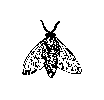
\includegraphics{fly}
\caption{A sample black and white graphic.}
\end{figure}

\begin{figure}
\centering
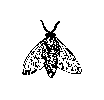
\includegraphics[height=1in, width=1in]{fly}
\caption{A sample black and white graphic
that has been resized with the \texttt{includegraphics} command.}
\end{figure}


As was the case with tables, you may want a figure
that spans two columns.  To do this, and still to
ensure proper ``floating'' placement of tables, use the environment
\textbf{figure*} to enclose the figure and its caption.
and don't forget to end the environment with
{figure*}, not {figure}!

\begin{figure*}
\centering
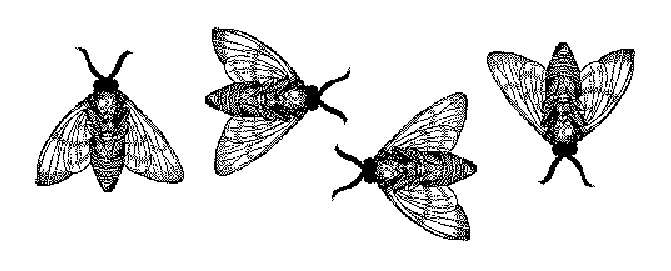
\includegraphics{flies}
\caption{A sample black and white graphic
that needs to span two columns of text.}
\end{figure*}


\begin{figure}
\centering
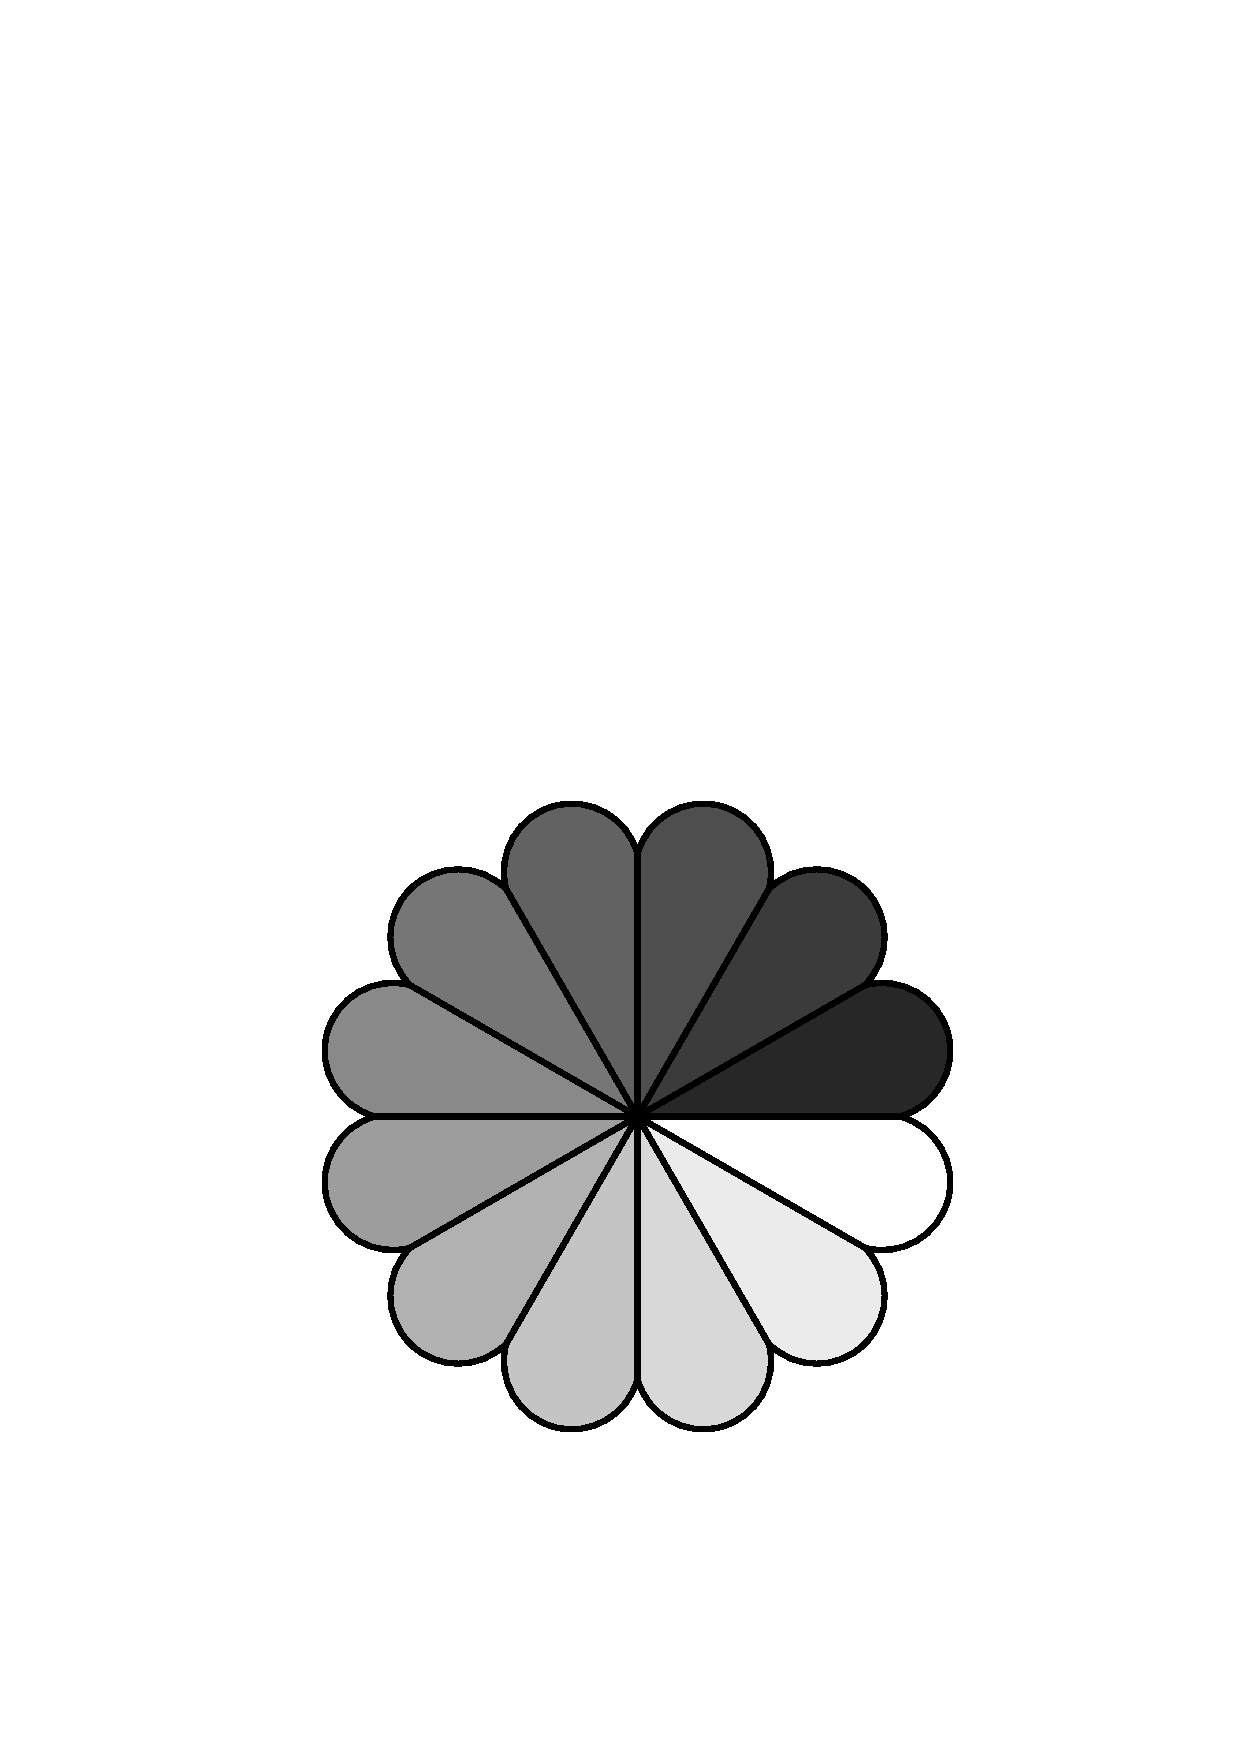
\includegraphics[height=1in, width=1in]{rosette}
\caption{A sample black and white graphic that has
been resized with the \texttt{includegraphics} command.}
\vskip -6pt
\end{figure}

\subsection{Theorem-like Constructs}
Other common constructs that may occur in your article are
the forms for logical constructs like theorems, axioms,
corollaries and proofs.  There are
two forms, one produced by the
command \texttt{{\char'134}newtheorem} and the
other by the command \texttt{{\char'134}newdef}; perhaps
the clearest and easiest way to distinguish them is
to compare the two in the output of this sample document:

This uses the \textbf{theorem} environment, created by
the\linebreak\texttt{{\char'134}newtheorem} command:
\newtheorem{theorem}{Theorem}
\begin{theorem}
Let $f$ be continuous on $[a,b]$.  If $G$ is
an antiderivative for $f$ on $[a,b]$, then
\begin{displaymath}\int^b_af(t)dt = G(b) - G(a).\end{displaymath}
\end{theorem}

The other uses the \textbf{definition} environment, created
by the \texttt{{\char'134}newdef} command:
\newdef{definition}{Definition}
\begin{definition}
If $z$ is irrational, then by $e^z$ we mean the
unique number which has
logarithm $z$: \begin{displaymath}{\log e^z = z}\end{displaymath}
\end{definition}

Two lists of constructs that use one of these
forms is given in the
\textit{Author's  Guidelines}.
 
There is one other similar construct environment, which is
already set up
for you; i.e. you must \textit{not} use
a \texttt{{\char'134}newdef} command to
create it: the \textbf{proof} environment.  Here
is a example of its use:
\begin{proof}
Suppose on the contrary there exists a real number $L$ such that
\begin{displaymath}
\lim_{x\rightarrow\infty} \frac{f(x)}{g(x)} = L.
\end{displaymath}
Then
\begin{displaymath}
l=\lim_{x\rightarrow c} f(x)
= \lim_{x\rightarrow c}
\left[ g{x} \cdot \frac{f(x)}{g(x)} \right ]
= \lim_{x\rightarrow c} g(x) \cdot \lim_{x\rightarrow c}
\frac{f(x)}{g(x)} = 0\cdot L = 0,
\end{displaymath}
which contradicts our assumption that $l\neq 0$.
\end{proof}

Complete rules about using these environments and using the
two different creation commands are in the
\textit{Author's Guide}; please consult it for more
detailed instructions.  If you need to use another construct,
not listed therein, which you want to have the same
formatting as the Theorem
or the Definition\cite{salas:calculus} shown above,
use the \texttt{{\char'134}newtheorem} or the
\texttt{{\char'134}newdef} command,
respectively, to create it.

\subsection*{A {\secit Caveat} for the \TeX\ Expert}
Because you have just been given permission to
use the \texttt{{\char'134}newdef} command to create a
new form, you might think you can
use \TeX's \texttt{{\char'134}def} to create a
new command: \textit{Please refrain from doing this!}
Remember that your \LaTeX\ source code is primarily intended
to create camera-ready copy, but may be converted
to other forms -- e.g. HTML. If you inadvertently omit
some or all of the \texttt{{\char'134}def}s recompilation will
be, to say the least, problematic.

\section{Background}
\label{sec:Background}

% Reference 3 types of agents that may be applicable to the project: 
% - Social Agents
% - Afective Agents
% - Anthromorphic Agents
% --- Embodied Conversational Agents (ECAs)

% When talking about trust and reputation mention the differences between both.
% Tell what is a trust model and what is a reputation model

Before discussing related work and our solution to the problem, we will present the main concepts that  will be mentioned in the rest of this report, specifically regarding Trust, Reputation and Game Theory.

\subsection{Trust}
\label{subsec:Trust}
Trust is regarded throughout the literature as one of the fundamental components of human society, being essential in cooperative and collaborative behaviour. So it has been studied in a multitude of disciplines, from Psychology and Sociology, to Philosophy and Economy\cite{Rousseau1998, Jones1997, Sabater2005}. For that reason, it is no wonder that it acquired a very large number of different definitions throughout the years of study, causing the problem of not existing a consensus on a definition of trust\cite{Castelfranchi2010}. But in the scope of this project, the most relevant basis is the dyadic definition of trust, where it is defined as: 'an orientation of an actor (the truster) toward a specific person (the trustee) with whom the actor is in some way interdependent' (taken from \cite{Simpson2007}), as we want to focus on interpersonal relationships. This definition has been expanded throughout the literature, often adapted to fit the context or scope of the work, but three main definitions were highlighted:
\begin{itemize}
	\tallitem First, Gambetta\cite{Gambetta1988} defined trust as follows: 'Trust is the \textit{subjective probability} by which an individual A, \textit{expects} that another individual, B, performs a given action on which its \textit{welfare depends}' (taken from \cite{Castelfranchi2010}). This is accepted by most authors as one of the most classical definitions of trust, but we agree with \cite{Castelfranchi2010}, in that it is restrictive it's uni-dimensionality, as it only refers to predictability of the trustor, and does not take into account competence in executing the given action.
	
	\tallitem Marsh\cite{Marsh1994} was the first author to formalize trust as a measurable Computational Concept, continuing the perspective of reducing trust to a numerical value, set by Gambetta\cite{Gambetta1988}, but also adding that: X trusts Y if, and only if, 'X \textit{expects} that Y will behave according to X's best interest, and will not attempt to harm X' (taken from \cite{Castelfranchi2010}). In this definition our opinions also match with \cite{Castelfranchi2010}, regarding that it does not represent other parts of trust, such as the notion that trustor must ascertain some risk from delegating the action to the trustee.
	
	\tallitem Castelfranchi and Falcone then defined a new definition and paradigm for Computational Trust, introducing a Cognitive aspect to it\cite{Castelfranchi1998}. They define Trust as the mental state of the trustor and the action in which the trustor refers upon the trustee to perform. This is the definition of trust that we will adopt throughout the rest of the report, as it represents a vision of trust that takes into account the trustor set of beliefs and intentions, approaching it to an agent's cognitive model, while also linking trust to the action being performed, as one might trust another for certain types of actions and not for others (e.g I may trust my squire to hold my sword, but not to swing it.).
\end{itemize}

\subsubsection{Castelfranchi and Falcone's Trust}
\label{subsubsec:CastelfranchiTrust}
More explicitly, Castelfranchi and Falcone\cite{Castelfranchi1998} state that Trust can be defined with a central core, composed by a five-part relation, between the trustor, the trustee, the context where they are inserted in, the action and outcome done by the trustee, and the goal of the trustor. This defines Trust as goal-oriented, contextual, and multi-dimensional, as from the point of view of the trustor, it varies not only on the trustee, but also from the overall context, the action the trustee is being delegated for, and the particular goal of the trustor. For example, if the goal of the trustor is simple to perform and not very critical to him, he may be more willing to delegate the task, and trust another agent to perform such task. It's important to note, that following this definition, Trust must imply that the trustor is taking some kind of risk by delegating a task to the trustee. Be it because the trustee may not able to perform the task, or that he may purposely ruin the task and go against the trustor goals.




\subsection{Reputation}
\label{subsec:Reputation}
Reputation is also a concept that appears very often linked with Trust in the literature, specially since most models created for representing trust have been focused on \acp{MAS}, where trust is influenced not only by the image one has of the subject, but also by what other agents say about it.

For the purpose of this report, reputation of an agent is defined as the combined trust opinion that the other agents that have manifested or provided about a particular subject. This reputation can and should be different from the individual image that various agents may have about the subject.


\subsection{Game Theory}
\label{subsec:GameTheory}
Game Theory is the field of study that defines and analyses situations involving conflict or cooperation between multiple intelligent decision makers. These situations are called a game, and they are distilled to their core argument, by defining the limited and simple set of actions that the players may perform, and how do they affect the players. It then analyses the decision strategies for each player, by assuming that both will try to maximise their payoff (how much the player gains) with their action. To better explain the concepts we want to present, we will introduce one of the most common exemplary models of Game Theory, the Prisoner's Dilemma.

\subsubsection{Prisoner's Dilemma}
\label{subsubsec:PrisonersDilemma}
The Prisoner's Dilemma is a two player game and is usually described as follows:

Two criminal partners are arrested and locked in separate cells with no way of communicating with each other. They are then questioned separately, where they are given 2 options, betray the other prisoner by testifying against him, or remain silent, with the following outcomes:
\begin{itemize}
	\item If both prisoners betray each other, both get 2 years in prison;
	\item If one of them betrays and the other remains silent, the betrayer goes free and the other gets 3 years in prison;
	\item If both remain silent, both get just 1 year in prison;
\end{itemize}

We can represent betraying as \textit{Defecting} (D), and staying silent as \textit{Cooperating} (C), and name the players \textit{player1} and \textit{player2}. So the game's possible outcomes can be represented by a payoff matrix, like the one in Table \ref{PrisonerDilemaPayoffMatrix} where each entry represents a tuple of the form (\textit{player1} payoff, \textit{player2} payoff). As the goal is to not get years in prison, the payoffs correspond to $Max\ years\ in\ prison - years\ got\ in\ prison$.

\begin{table}[]
	\centering
	\begin{tabular}{l|l|l|}
		\cline{2-3}
		& $C_2$   & $D_2$   \\ \hline
		\multicolumn{1}{|l|}{$C_1$} & 2,2 & 0,3 \\ \hline
		\multicolumn{1}{|l|}{$D_1$} & 3,0 & 1,1 \\ \hline
	\end{tabular}
	\caption{Prisoner's Dilemma Payoff Matrix}
	\label{PrisonerDilemaPayoffMatrix}
\end{table}	

In the game we can say that \textit{Defecting} \textbf{dominates} \textit{Cooperating}, as for any action that the adversary player may choose, \textit{Defecting} always gives a better payoff for the individual player.\cite{Nash1951} So a rational player will never choose to \textit{Cooperate}.


% More than a literature review
% Organize related work - impose structure
% Be clear as to how previous work being described relates to your own.
% The reader should not be left wondering why you've described something!!
% Critique the existing work - Where is it strong where is it weak? What are the unreasonable/undesirable assumptions?
% Identify opportunities for more research (i.e., your thesis) Are there unaddressed, or more important related topics?
% After reading this chapter, one should understand the motivation for and importance of your thesis
% You should clearly and precisely define all of the key concepts dealt with in the rest of the thesis, and teach the reader what s/he needs to know to understand the rest of the thesis.


\section{Related Work}
\label{sec:Related Work}
Computational Trust research has been focused on modelling trust in \acp{MAS}, specially on open e-commerce environments\cite{Granatyr2015, HanYu2013, Pinyol2013, Noorian2010, Huang2008}, with at least 106 models created\cite{Granatyr2015}, since the formalization of trust as a measurable property by Marsh in 1994 \cite{Marsh1994}. We will present some trust models from which we will take inspiration while creating our own, and some work done in measuring trust in \ac{HRI}.

\subsection{Trust Models}
\label{subsec:Related work:Trust Models}
For related work concerning Trust Models we will focus on \textbf{Cognitive} Trust Models, first introduced by Castelfranchi and Falcone\cite{Castelfranchi1998}, as we want to focus on modelling trust through multiple dimensions, with the intent of having trust depend on the action to perform, context and agent performing the task and having these dimensions represented explicitly in the model, something that it is not possible with \textbf{Numerical}, like the one introduced by \cite{Marsh1994}.

\subsubsection{Castelfranchi and Falcone}
Having developed the concept of Cognitive Trust Models, this author's model is generally regarded as a classical basis for most other authors, and while we will not use this model directly, it is worth describing it in this report, as it was also a source of inspiration to other authors referenced in this report. 
The model is characterised around their definition referred in Section \ref{subsubsec:CastelfranchiTrust}, through a central core, composed by a five-part relation, between:
\begin{itemize}
	\item the trustor (\textbf{X});
	\item the trustee (\textbf{Y});
	\item the context where they are inserted in (\textbf{C});
\end{itemize}
	 a pair composed action and outcome done by the trustee, and the goal of the trustor. This defines Trust as goal-oriented, contextual, and multi-dimensional, as from the point of view of the trustor, it varies not only on the trustee, but also from the overall context, the action that is being delegated, and the particular goal of the trustor. For example, if the goal of the trustor is simple to perform and not very critical to him, he may be more willing to delegate the task, and trust another agent to perform such task. Adjustments can be attached to this core adjusting better to the context in which it may be used. For instance, one may add an authoritative third party element to the relation in supervised security applications.

\begin{equation}
	TRUST(X\ Y\ C\ \tau\ g_x)
	\label{eq:TrustRelation}
\end{equation}

 quantifies trust by defining \textbf{Degrees of Trust} 


\subsubsection{Repage}


\subsubsection{BDI + Repage}

\subsection{The Perception and Measurement of Human-Robot Trust}
\label{subsec:Related work:The Perception and Measurement of Human-Robot Trust}

Schaefer\cite{Schaefer2009} presents a trust perception scale, that provides a way of extracting an accurate trust score from humans interacting with robots. The scale is composed of 40 items that can be ranked from 0 to 100, in 10 point intervals. The final result it then averaged by adding all the item values and divided by the total number of items (40).



While this work has been done specifically for \ac{HRI} we believe that a sub-set of this items can be used for the features used in the cognitive model of the user's trust, further described in Section %todo give refence here





% O que fizeram?
% Como se enquadra?
% Porque é importante?
% Como pode ser útil?

\subsection{Discussion}
\label{subsec:RelWorkDiscussion}

Based on everything and what everyone is doing or done, these are the problems, these are the advantageous and disavantageous of the aproach.
% This is "Conclusions.tex"
% A content sub-file of "TrustfullActionSugestion-Paper.tex"
\section{Conclusions}
Throughout this paper we addressed the work done to develop a Cognitive Trust Model capable of suggesting actions to improve Trust on a virtual agent. We first went through our thoughts about the lack of research done in the area of trust in \ac{HRI}, especially regarding trust improvement, and what we propose to address that issue. Then we went on to establish some background in \ac{HRI} concepts specific to the domain, like the various definitions of Trust, while going through some discussion as what was more appropriate for our work. In the next chapter we delved into some of the MAS trust models that we found. While there were many more aside from those discussed in this thesis, we wanted to focus on the ones that followed the Cognitive trust paradigm and most closely related with the one we developed. Following that we presented our Trust Model, describing its 3 main components: Memory, Perception and Action Suggestion, and how they interact to compose our model. Due to problems finding a suitable evaluation scenario for our model, we then describe our second contribution of this thesis, a novel Trust and Rapport evaluation scenario, Quick Numbers, that aims to address the willingness factor of trust, by imposing to the participant the choice to entrust the agent with their own earned resources. Finally we showed how used the scenario to perform User Studies on the Trust Model. Unfortunately, the results can be considered either inconclusive or right against our effort to improve Trust, as there was no apparent change in Trust measurements in conditions with and without the Action Suggestion module. Nevertheless, we believe that our efforts were significant by providing an implementable base from which other research projects in the same area may start. 

%\end{document}  % This is where a 'short' article might terminate

%ACKNOWLEDGMENTS are optional
% This is "Acknowledgments.tex"
% A content sub-file for Trustfull Action Suggestion Thesis Extended Abstract
\section{Acknowledgments}
This section is optional; it is a location for you
to acknowledge grants, funding, editing assistance and
what have you.  In the present case, for example, the
authors would like to thank Gerald Murray of ACM for
his help in codifying this \textit{Author's Guide}
and the \textbf{.cls} and \textbf{.tex} files that it describes.
%
% The following two commands are all you need in the
% initial runs of your .tex file to
% produce the bibliography for the citations in your paper.
\bibliographystyle{abbrv}
\bibliography{bib/sigproc}  % sigproc.bib is the name of the Bibliography in this case
% You must have a proper ".bib" file
%  and remember to run:
% latex bibtex latex latex
% to resolve all references
%
% ACM needs 'a single self-contained file'!
%
%APPENDICES are optional
%\balancecolumns
\appendix
\section*{Appendices}
\section{Variants of Single-subject designs}

\newpage
\begin{landscape}
	\section{Landscape Appendice}
	\label{app:Educational}	
	landscape page
\end{landscape}

\newpage
\section{The Perception and Measurement of Human-Robot Trust: Items Table}

\begin{longtable}{l|l}
	\multicolumn{1}{c|}{\textbf{Items}} & \textbf{Perceived as relevant} \\ \hline
	\endhead
	Act consistently & \\ \hline
	Protect people & \\ \hline
	Act as part of the team & \\ \hline
	Function successfully & \\ \hline
	Malfunction & \\ \hline
	Clearly communicate & \\ \hline
	Require frequent maintenance & \\ \hline
	Openly communicate & \\ \hline
	Have errors & \\ \hline
	Perform a task better than a novice human user & \\ \hline
	Know the difference between friend and foe & \\ \hline
	Provide Feedback & \\ \hline
	Possess adequate decision- making capability & \\ \hline
	Warn people of potential risks in the environment & \\ \hline
	Meet the needs of the mission & \\ \hline
	Provide appropriate information & \\ \hline
	Communicate with people & \\ \hline
	Work best with a team & \\ \hline
	Keep classified information secure & \\ \hline
	Perform exactly as instructed & \\ \hline
	Make sensible decisions & \\ \hline
	Work in close proximity with people & \\ \hline
	Tell the truth & \\ \hline
	Perform many functions at one time & \\ \hline
	Follow directions & \\ \hline
	Considered part of the team & \\ \hline
	Responsible & \\ \hline
	Supportive & \\ \hline
	Incompetent & \\ \hline
	Dependable & \\ \hline
	Friendly & \\ \hline
	Reliable & \\ \hline
	Pleasant & \\ \hline
	Unresponsive & \\ \hline
	Autonomous & \\ \hline
	Predictable & \\ \hline
	Conscious & \\ \hline
	Lifelike & \\ \hline
	A good teammate & \\ \hline
	Led astray by unexpected changes in the environment & \\
	\caption{The Perception and Measurement of Human-Robot Trust: Items Table}
	\label{app:measurement.items.table}	
\end{longtable}


%\balancecolumns % GM June 2007
% That's all folks!
\end{document}
